%----------------------------------------------------------------------------
\chapter{Garage Gate}\label{sect:garage-statechart}
%----------------------------------------------------------------------------
\section{State machine introduction}
%----------------------------------------------------------------------------

A garage gate fundamentally have 2 main states, the \textit{Opened} and \textit{Closed} states, which is shown below on \figref{Garage State machine} figure, with orange colors. First of all we can start from the \textit{Closed} state, where we can open the gate with an 'open' command. This command sets the state machine in an \textit{Opening} state. While opening the gate, somebody or something can move into the way, so this becomes \textit{Block Opening}. The gate is opening, if the blocking stops. After the \textit{Opening} phase succeded the gate is \textit{Opened}. In this state we can 'close' the gate with a simple command, and the state machine goes to the \textit{Closing} state. There could be also a blocking action, which stops the closing movement. From this state the gate is starting the closing movement again after a few seconds \textit{Lighting}. When the closing action finished the gate is \textit{Closed}

\begin{figure}[!ht]
\centering
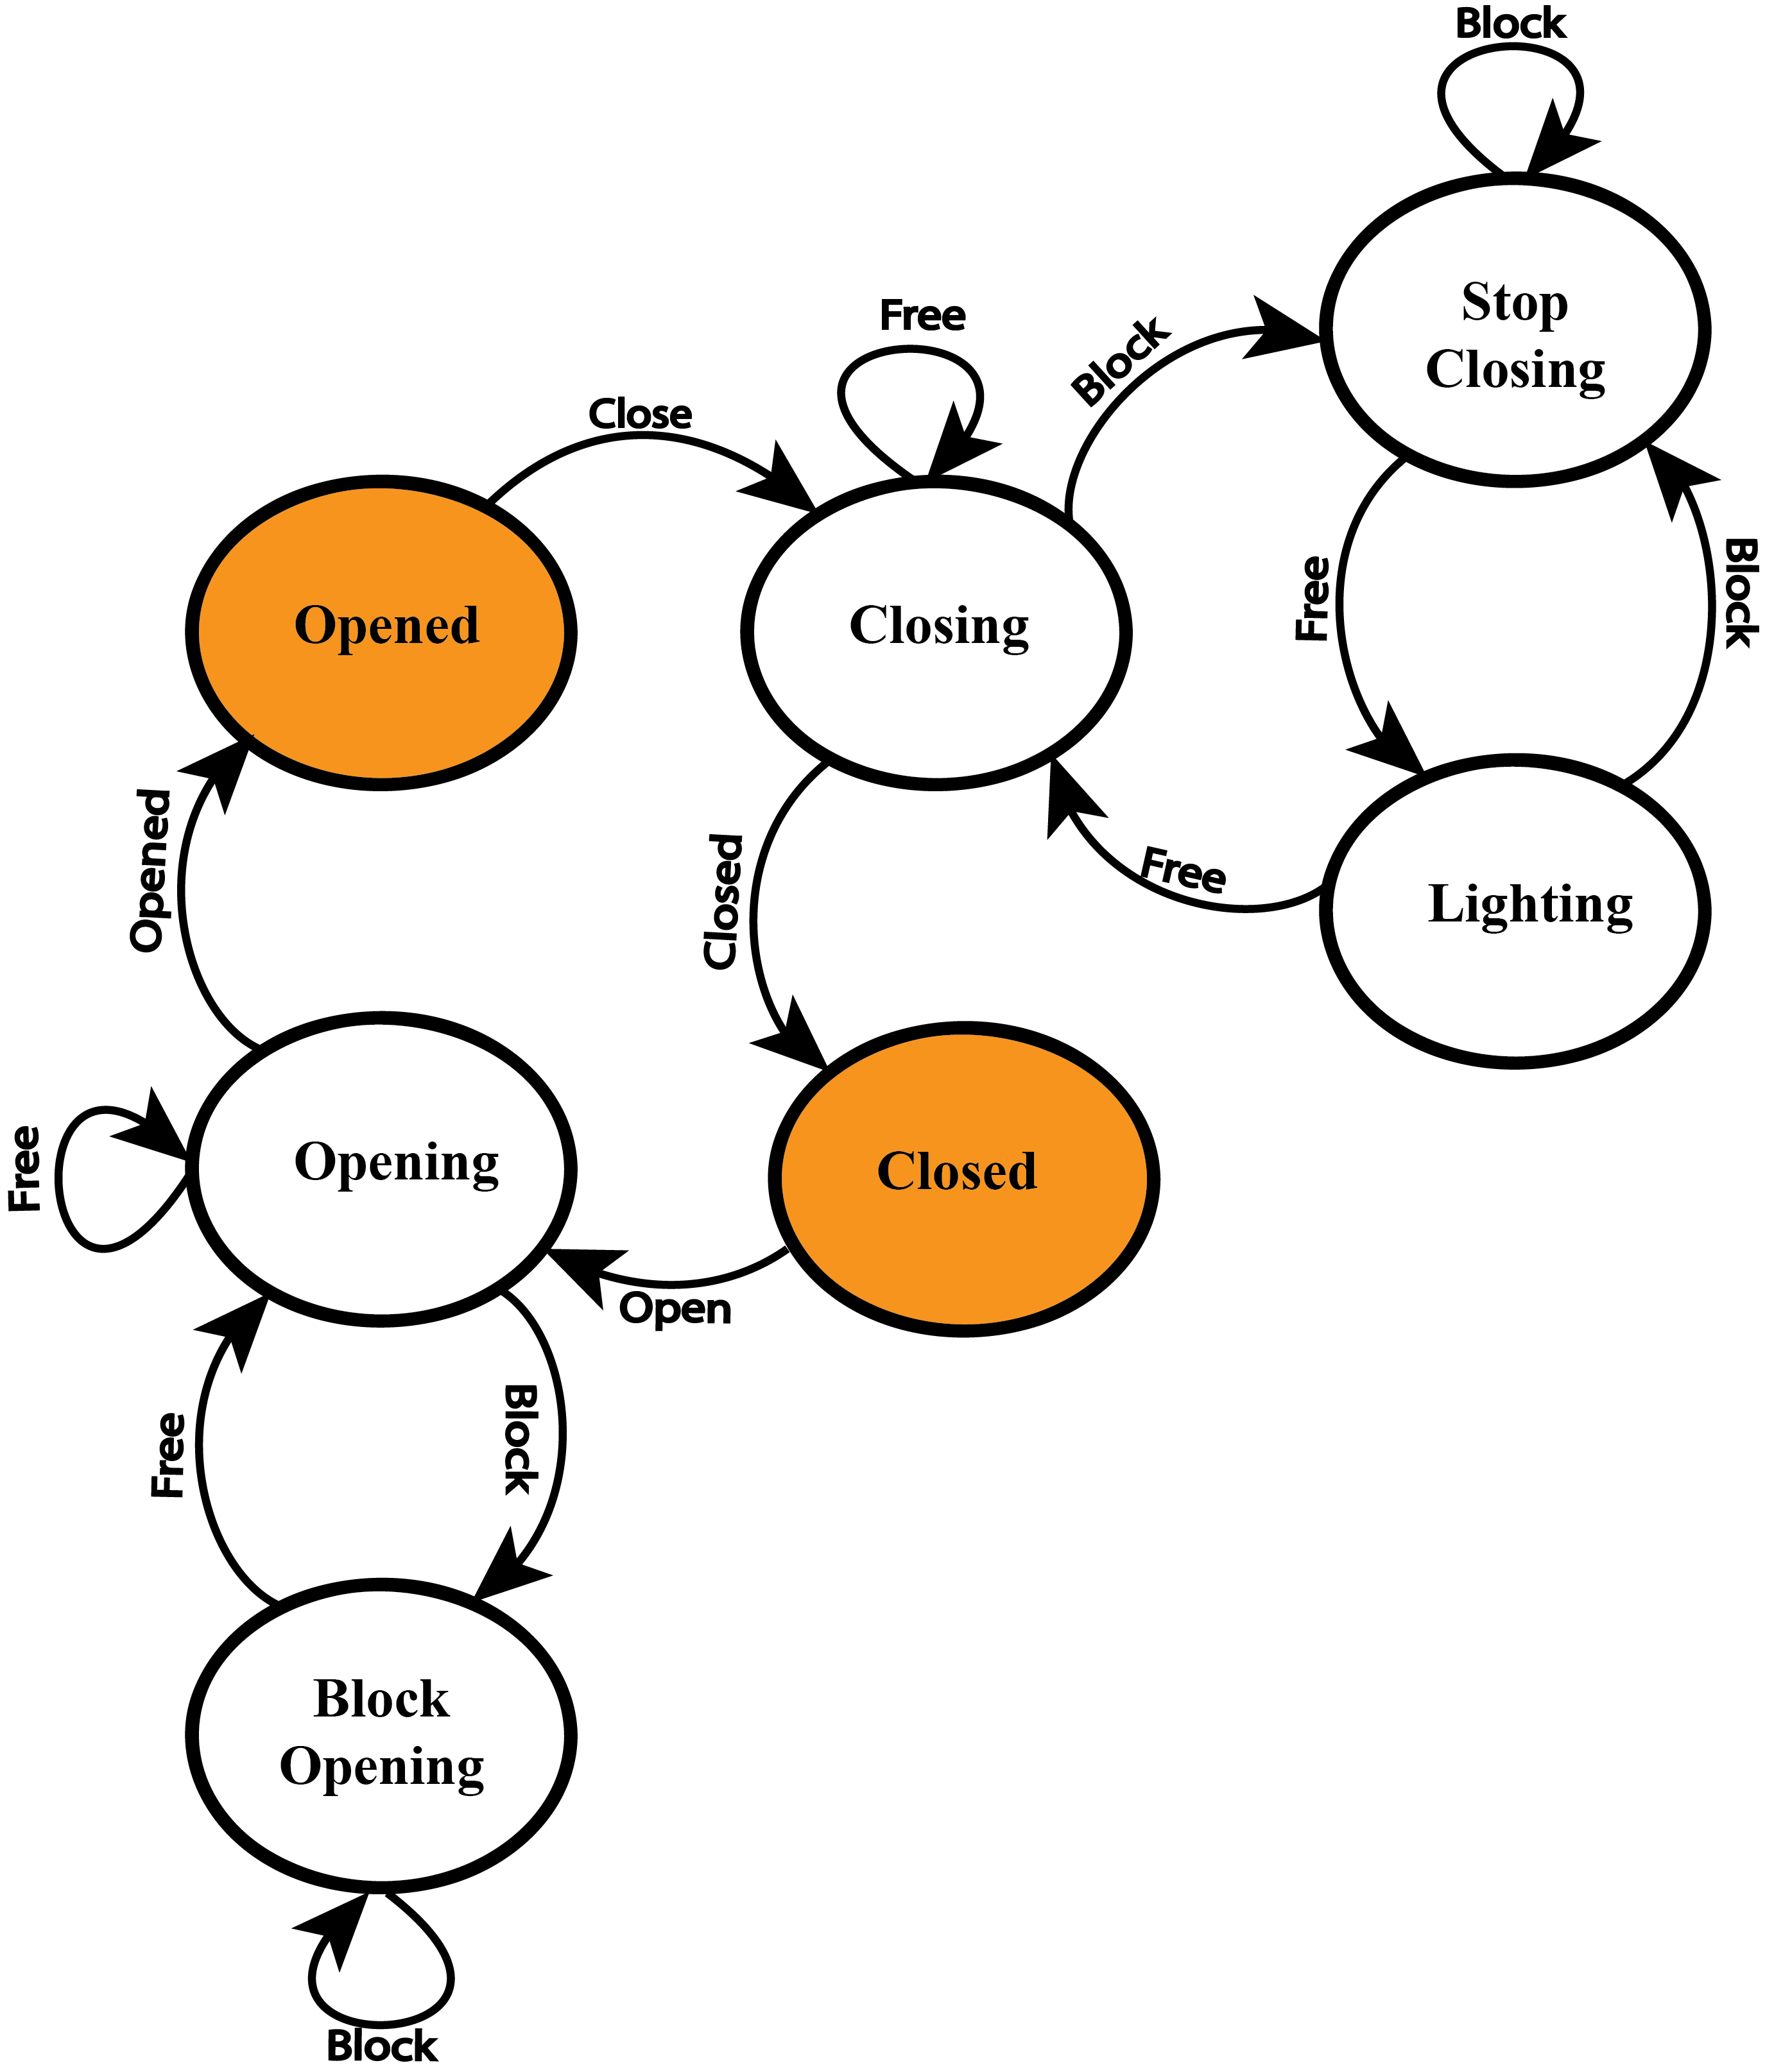
\includegraphics[width=150mm, keepaspectratio]{figures/garage.png}
\caption{The garage gate statechart.}
\label{fig:Garage Statechart}
\end{figure}
